\documentclass[tikz,border=2pt]{standalone}
\usepackage{amsmath,amssymb}
\usepackage{tikz}
\usetikzlibrary{arrows.meta,matrix}

\begin{document}
% Row echelon form is a staircase: each pivot sits strictly to the right of the pivot above,
% zero rows at the bottom. Reduced form additionally has pivots equal to 1 with zeros above.
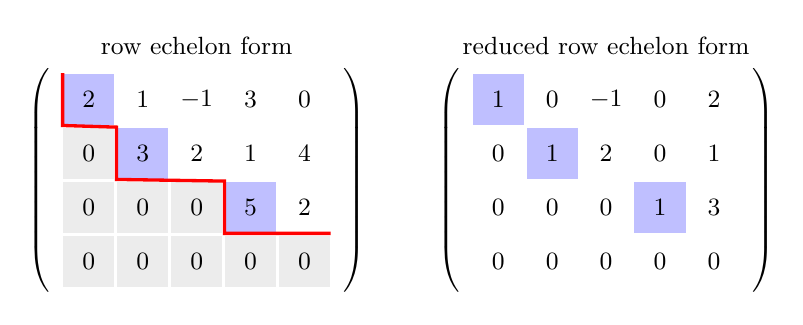
\begin{tikzpicture}[every node/.style={font=\small}]
	\matrix (A) [matrix of math nodes, nodes={minimum size=6.5mm, anchor=center}, left delimiter=(, right delimiter=), column sep=1pt, row sep=1pt] at (0,0) {
		|[fill=blue!25]| 2 & 1 & -1 & 3 & 0 \\
		|[fill=gray!15]| 0 & |[fill=blue!25]| 3 & 2 & 1 & 4 \\
		|[fill=gray!15]| 0 & |[fill=gray!15]| 0 & |[fill=gray!15]| 0 & |[fill=blue!25]| 5 & 2 \\
		|[fill=gray!15]| 0 & |[fill=gray!15]| 0 & |[fill=gray!15]| 0 & |[fill=gray!15]| 0 & |[fill=gray!15]| 0 \\
	};
	\draw[red, very thick] (A-1-1.north west) -- (A-1-1.south west) -- (A-2-2.north west) -- (A-2-2.south west) -- (A-3-4.north west) -- (A-3-4.south west) -- (A-3-5.south east);
	\node[anchor=south] at (A.north) {row echelon form};
	\matrix (R) [matrix of math nodes, nodes={minimum size=6.5mm, anchor=center}, left delimiter=(, right delimiter=), column sep=1pt, row sep=1pt] at (5.2,0) {
		|[fill=blue!25]| 1 & 0 & -1 & 0 & 2 \\
		0 & |[fill=blue!25]| 1 & 2 & 0 & 1 \\
		0 & 0 & 0 & |[fill=blue!25]| 1 & 3 \\
		0 & 0 & 0 & 0 & 0 \\
	};
	\node[anchor=south] at (R.north) {reduced row echelon form};
\end{tikzpicture}
\end{document}
